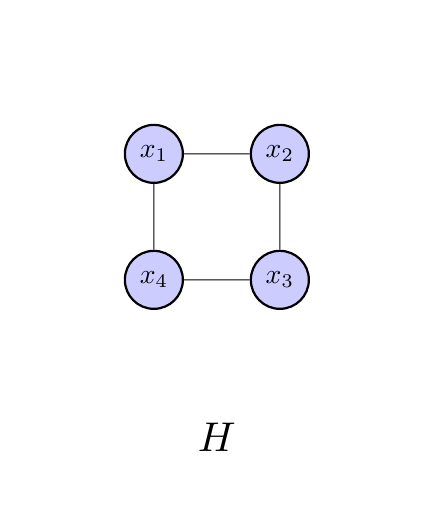
\begin{tikzpicture}[scale=.8,auto=left,every node/.style={circle,fill=blue!20,draw=black,thick}]
  % Vértices del cuadrado interior (C_4)
   \node (w1) at (-1, 1) {$x_1$};
  \node (w2) at (1, 1) {$x_2$};
  \node (w3) at (1, -1) {$x_3$};
  \node (w4) at (-1, -1) {$x_4$};

  % Vértices del cuadrado exterior (C_4 más grande)
  \node (w5) at (-2.5, 2.5) [opacity=0]{$w_5$};
  \node (w6) at (2.5, 2.5) [opacity=0]{$w_6$};
  \node (w7) at (2.5, -2.5) [opacity=0]{$w_7$};
  \node (w8) at (-2.5, -2.5) [opacity=0]{$w_8$};

  % Aristas del cuadrado interior
  \foreach \from/\to in {w1/w2, w2/w3, w3/w4, w4/w1}
    \draw (\from) -- (\to);

  % Título del grafo en la parte inferior
  \node[draw=none, fill=none, scale=1.5] at (0,-3.5) {$H$};
\end{tikzpicture}
